\section{Design}
\ninanotes{
\begin{itemize}
\item Design
\item How is the solution constructed, on which design elements?
\item Which components does the solution consist of?
\item Which technologies, tools or packages are used?
\item Discuss alternatives and motivate your choice.
\end{itemize}
}
\newcommand{\POVModel}{\mathcal{M}}

% \subsection{Representing a card and deck compactly}
% Since a single card cannot take more one of 25 different, then enumerating each card, a single Card type needs 5 bits in order to reperesent a value.





Given the constraints on time and space, it would be nice to have a quite compact representation of each world, furthermore, given that query algorithms will go through most (if not all) of the possible worlds, iterating though the possible worlds should be fast. A fast way to iterate through elements is to make sure that each element is small as well as contiguous in order to make use of the CPUs caching system the most, i.e. small elements in a contiguous data structure which guarantees good spatial locality.


\subsection{Formalizing accessing in a model} \label{sec:model-access}
In order to get good spatial locality I want to explain how to take the model from section \ref{sec:description-of-how-modal-logic-is_applied} and describe how it might be turned into an array.

In the section \ref{sec:description-of-how-modal-logic-is_applied} I went through the overall approach of generating the worlds from a specific agents POV. In order to specify how such worlds might be accessed, I extend the solution with some notation. Let $\POVModel_p: W \rightarrow P \rightarrow \mathcal{P}(W)$ be the model for the player $p$'s POV. Here the interpretation is that the model takes some fixed scenario $w$ of type $W$, and some player $b$ of type $P$, then we have all the worlds that $p$ cannot rule out that $b$ finds possible, given that $w$ is the case. Of course if $b=p$ then we have the unit set, which is simply $\POVModel_p(w)(p) = \{w\}$. Which also makes sense in the interpretation "given that we fix the world to $w$, then player $p$ can only imagine that $p$'s only possible world is $w$". 

It is clear from the above mapping that this could be encoded using a 3-dimensional array. Where $W$ (the first argument) could be an enumeration of the possible worlds for $p$, and $P$ could be an enumeration of the players, and $\mathcal{P}(W)$ could be an array of possible worlds.



\subsection{Representing the world} \label{sec:representing-a-world}
A world is simply a possible state of the entire game, i.e. everything is specified, including the hands you can't see. A naive approach to representing a world is to take the deck, the discard pile, all of the hands etc. into account. But this approach is definitely more than necessary, since what is in the discard pile and in the color pile, as well as most hands, are information easily accessed by the agents themselves, by checking the current state of affairs. Furthermore I choose not to take order into account in any of the hands or piles, because it would lead to too many combinations (a hand of 4 cards has 25 permutations, assuming that all are unique). What is most interesting to represent is simply then what is uncertain. So in this case it is a player's own hand and the deck. Of course assuming some hand will give an unambigous content of the deck, and vice versa, so it is sufficient to just represent the unknown hand. So a query $\POVModel_p(w)(b)$, will return the set of hands that $p$ cannot rule out that $b$ believes, given that the hand $w$ is the case for $p$.

There are various approaching to representing a hand, I will go through a few I have deviced. 

\begin{enumerate}
\item Represent each card in a sorted order. Called sorted-order representation
\item Enumerate each possible hand. Called Enumeration representation
\item Contingency table inspired set. Called table representation.
\end{enumerate}

In each representation I will go through the number of theoretical bits needed per world as well as what the actual number of bits are if we have to make it directly byte-addressable. The reason I write "theoretical" is due to that most CPU architectures (as well as how Zig compiles code \cite{zigdocspackedstruct}) are byte-addressable. This means that the smallest adressable space is 1 byte on most modern architectures, even if you want to represent something that uses fewer bits. The theoretical number of bits can be reached, but will require some packing of structs or bitmanipulation, and comes with the tradeoff of more CPU cycles spent on bitmasking the value rather than simply accessing it. 


\paragraph{Represent each card in a sorted order}
So firstly we want to look at how small can we get away with representing a card. A card can be one of 25 different instances (5 suits times 5 values), so a minimal representation could enumerate each card and a world be represented by 5 bits (which can represent from 32 different values).
Then if we have a hand of 4 cards, that means we spent $4 \frac{\text{cards}}{\text{hand}} \cdot 5 \frac{\text{bits}}{\text{cards}} = 20 \frac{\text{bits}}{\text{hand}}$. And using the same reasoning we use 25 bits for 5 cards.
Then we can predefine some sorted order of the 25 different instances, and just sort a hand in order to get its set representation.

If each card has to be byte-addressable then it would have to use 1 byte (8 bits), which would then mean that a hand of 4 cards is 24 bits, and a hand of 5 cards is 40 bits.

Pros: Very simple and compact representation. No obvious cons.

\paragraph{Enumerate each possible hand}
If you draw 4 cards blindly from an initial deck of 50 cards, there are 18480 distinct combinations (data from Appendix \ref{appendix:python-distinct-combinations}). If it 5 cards drawn it is 99455. 
Depending on the situation, you could enumerate each possible hand. Then a world need only an integer size large enough to store 18480 or 99455 depending on the case. This is respectively 15 bits and 17 bits.
So this representation is definitely compact. Of course some edge-cases exists, for instance in a 5 player game, when the last card has been drawn, then there can exist both 4 and 5 cards representations at the same time, but that would require bits enough to represent $18480+99455 = 117935 < 2^{17}$ so 17 bits should still be sufficient.

Of course if the representation would have to be byte-addressable in an array, then it would have to spent a whole number of bytes, which is repectively 2 bytes (16 bits) or 3 bytes (24 bits).

Of course this enumeration would only create a mapping from an integer to an actual representation, so we would still have to choose a representation that this integer maps to. Which can be either sorted-order or table representation

Pros: Very compact representation, the enumeration map should only take some constant amount of memory at all times. Even if we assume the worst case, which is using the table representation and enumerating

Cons: Non-trivial to implement. A lot of conversion between values i.e. its hard to work on a world directly without looking it up in a map, so when iterating through a list of possible worlds I will have to look up what that world actually is, this I imagine will substantially slow down the algorithm, although I have not tested it.

\paragraph{Contingency table inspired set}
This representation I stumpled upon when trying to figure out how to generate the possible hands in a fast manner (more on the generation in section \ref{sec:efficient-generation-of-hands}).
Given that instance of a card can at most occur 3 times in a hand (or deck for that matter). Then an array of 25 elements, each element being able to store 0 through 3, will be a sufficient representation. This means that each element in the array need only be 2 bits. So a theoretic use of space is $2 \frac{\text{bits}}{\text{elements}} \cdot 25\text{elements} = 50$ bits. 

If each element has to be byte-addressable then it will have to spent 1 byte per element, in which case $8 \frac{\text{bits}}{\text{elements}} \cdot 25\text{elements} = 200$ bits. Which is a pretty big increase from the theoretical 50 bits.  

Pros: Very direct set representation of the cards, can even be used for the piles and deck. 

Cons: Spents a lot more bits than strictly necessary to represent a world.


\subsubsection{Choosing a representation}
All representations have a convincing set of of tradeoffs. I decided to go with the table representation, since it is very generalizable for other aspects of the game (i.e. can be used to represent decks, piles etc.), as well as easy to work on directly, as well as generate, see section \ref{sec:efficient-generation-of-hands}. 
But the other representations should definitely be kept in mind if memory proves to be a problem in practice.


\subsection{Generating hands in an efficient way} \label{sec:efficient-generation-of-hands}
Using the methods described in math.stackexchange posts "Efficient algorithm to find all unique combinations of set given duplicates" \cite{HardmathcontigencyTablePost} and \cite{GCabrecursiveGenerationPost}, I was able to design a good generation method for the hands. 
The main idea is that we represent the hands we want to generate in a contingency table, where we have some pool to take from. So a case with handsize set to 0 and the pool being the initial deck will be Figure \ref{fig:hand-pool-table} (of course in a practical game, you would know something about the other hands and the discard pile etc. so the pool would be less than the initial deck). Then the problem is to generate all such contingency tables, such that the sum of the hand is $k$ (usually 4 or 5), and the column sums stay the same, for example see Figure \ref{fig:hand-pool-table-with-hand}.

\begin{figure}
	\centering
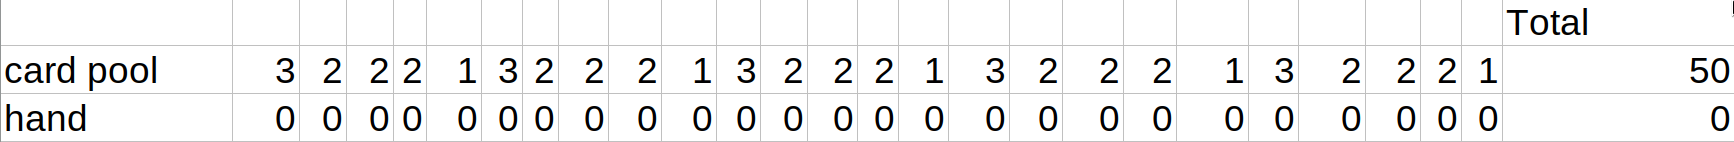
\includegraphics[width=13cm,frame]{images/contigency_table.png}
	\caption{Contingency table with handsize set to 0}
	\label{fig:hand-pool-table}
\end{figure}


\begin{figure}
	\centering
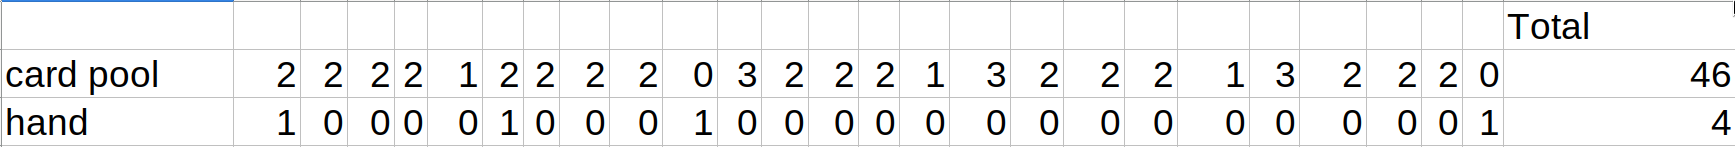
\includegraphics[width=13cm,frame]{images/contigency_table_with_hand.png}
	\caption{Contingency table with handsize set to 4}
	\label{fig:hand-pool-table-with-hand}
\end{figure}

Both the card pool and the hand can be represented by using the table representation described in section \ref{sec:representing-a-world}.

The simplest way to describe how the hand is generated, is to view the hand table entries as digits in an integer (or more mathematically specific, a multi-radix integer), with the leftmost digit being the most significant, and then you create the biggest integer with cross-sum $k$, and subsequently construct the number just below that, still with constraint that the cross-sum must be $k$. So continuing the example with Figure \ref{fig:hand-pool-table}, we can create the "biggest integer" in this way Figure \ref{fig:biggest-integer}. Then the integer just below that is Figure \ref{fig:next-integer}. And continuing with 1s until we get Figure \ref{fig:etc-one}.
Then we decrement the most signficant digit and get Figure \ref{fig:decrement}.

\begin{figure}
	\centering
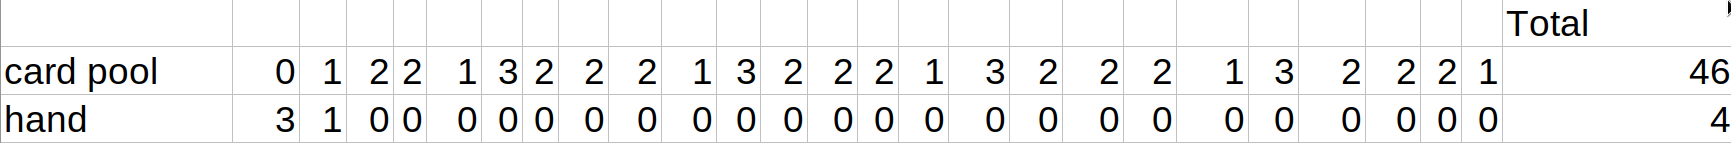
\includegraphics[width=13cm,frame]{images/biggest_integer.png}
	\caption{First generated hand}
	\label{fig:biggest-integer}
\end{figure}

\begin{figure}
	\centering
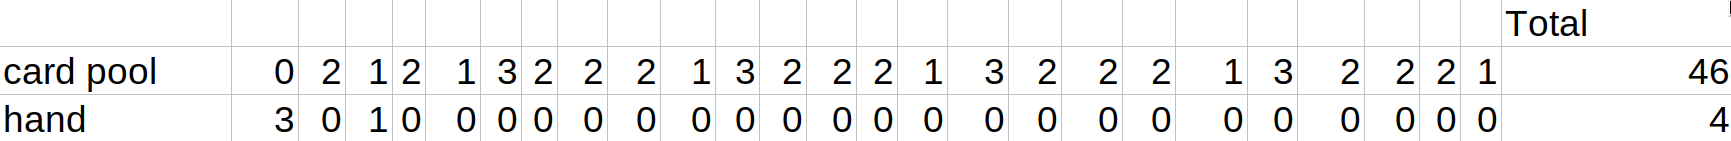
\includegraphics[width=13cm,frame]{images/next-biggest.png}
	\caption{Second generated hand}
	\label{fig:next-integer}
\end{figure}

\begin{figure}
	\centering
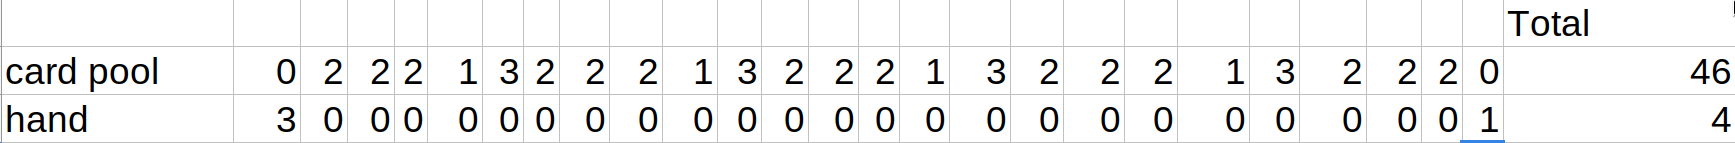
\includegraphics[width=13cm,frame]{images/etc_one.png}
	\caption{The smallest integer containing 3 in the first position}
	\label{fig:etc-one}
\end{figure}


\begin{figure}
	\centering
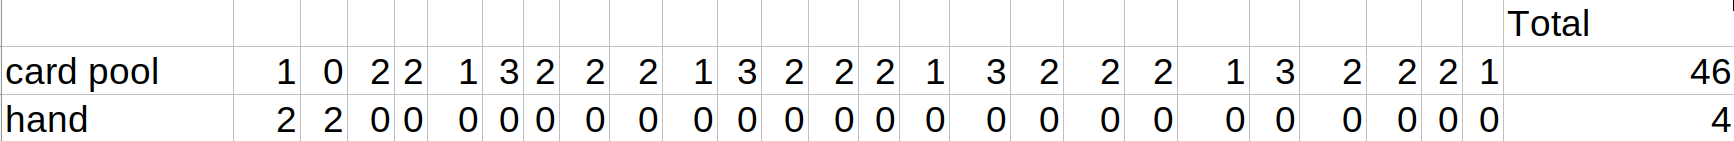
\includegraphics[width=13cm,frame]{images/decrement.png}
	\caption{The biggest integer containing 2 in the first position}
	\label{fig:decrement}
\end{figure}


A more formalized algorithmic approach will be described in the implementation chapter.


\subsection{How should an agent play?} \label{sec:how-should-an-agent-play}

How an agent should play based on its knowledge in its DEL model is heavily inspired by \cite{CoxEtAl2015}, specifically the "information strategy". 
In it they distinguish between \emph{public and private information}. Where public information is what everybody knows, and everybody knows that everybody knows that etc. And private information, is what an agent individually knows based on the other players hands. This can be compared to DEL where public information is what the model guarantees is common knowledge, and private information is simply queries that holds true for all possible worlds from that agents POV.

In my solution I will only look at private information, but it is an interesting problem to see how one can adapt the model I have described into something that can answer common knowledge queries, especially given that \cite{CoxEtAl2015} information strategy makes use of common knowledge.

In order to decide what an agent should do in a specific situation, I borrow terminology from \cite{CoxEtAl2015} again. So given a hand, which is a ordered set of known or unknown cards, how does an agent know what card to play?


% In order to decide what an agent should do in a specific situation, I borrow terminology from \cite{CoxEtAl2015} again. So given a hand, which is a ordered set of known or unknown cards

% However the private information my agents got is not the tables defined in \cite{CoxEtAl2015}, but the DEL model described in section \ref{sec:model-access}. The action algorithm for the information strategy is as follows (most of it cited directly from \cite{CoxEtAl2015}):

% Adapting \cite{CoxEtAl2015} information strategy to the model I have described is pretty straight-forward. 

Firstly I will have to decide \emph{when} a card should be played, discarded etc. Here I use the action algorithm from \cite{CoxEtAl2015}:
\begin{enumerate}
	\item Play the playable card with lowest index.
	\item If there are less than 5 cards in the discard pile, discard the dead card with lowest index.
	\item If there are hint tokens available, give a hint.
	\item Discard the dead card with lowest index.
	\item If a card in the player’s hand is the same as another card in any player’s hand, i.e.,it is a duplicate, discard that card.
	\item Discard the dispensable card with lowest index.
	\item Discard index 0.
\end{enumerate}

Here implicitly "playable card", "dispensible card", "dead card", "it is a duplicate", are epistemic queries on the $\POVModel_p$ for the current playing player $p$'s hand. So how would an agent go about trying to decide whether a card is playable, discardable, dead, a duplicate or dispensible? Let's denote each of these the cards \emph{actionable states}.

I define the actionable states is as follows (also based on \cite{CoxEtAl2015}):
\begin{itemize}
	\item Playable: If it is able to be played in the current game state.
	\item Dead: If the card has already been played and is not needed anymore.
	\item Dispensible: If the card could be played at some point (now or in the future), but there is at least one more of the same card left.
	\item Duplicate: There exists duplicate in another players hand.
\end{itemize}

The problem with deciding actionable states for the cards is that we have stored each world as a set, and since a set ignores order of the cards, then even if we find hands with several actionable states in the model, we still have to find a mapping between the set and the ordered list that is the concrete hand that the agent is playing with.
So for the agent's POV, the hand the player has can be viewed as an ordered list of what is hinted about the agent's cards. What is known about a card can be denoted by a pair: its suit, and its value. 

As an example: If I have the hand ((red,1),(blue,3),(red,2),(yellow,3)), and the current state of the game I have only my red cards hinted, then the ordered list $o_{hints}$ is (red,unknown),(unknown,unknown),(red,unknown),(unknown,unknown).

In order to create the mapping from a set in a world to an ordered list that matches the hand indices, we have to take the hints given to player $p$ into account.
So given an unknown hand for player $p$ specified with the ordered list of hints $o_{hints}$, and the model $\POVModel_p$ we have to decide what possible actionable states is in each card. 

For each possible world for $p$, there is a specific hand for $p$, denoted $h_{specific}$. Since each hand is stored as a set, we have to use the hints $o_{hints}$ to figure out how the set should be mapped to ordered list. How this can be done is to make $h_{specific}$ into any ordered list $o_{specific}$ and subsequently take all permutations of $o_{specific}$ and see which ones matches the $h_{hints}$. If it is possible to find any permutation that is non-contradictory with $o_{hints}$ then we can decide the actionable states for each card given by $h_{specific}$.

Continuing the previous example. We might have the set \[h_{specific} = \{(green,1),(red,5),(green,2),(red,1)\}\]
Turning this into an ordered list 
\[o_{specific} = ((green,1),(red,5),(green,2),(red,1))\]
we see that there are 4 permutation that matches $o_{hints}$:

\[o_{1} = ((red,5),(green,1),(red,1),(green,2))\]
\[o_{2} = ((red,1),(green,1),(red,5),(green,2))\]
\[o_{3} = ((red,5),(green,2),(red,1),(green,1))\]
\[o_{4} = ((red,1),(green,2),(red,5),(green,1))\]

Then for each permutation we can decide the actionable states of each card, based on the permutation and the current state of the game. For instance, let us assume that the red color pile in the current state of the game has a 4 on top. This means that the card in position 0 can both be playable (if it is a (red,5)). But it is also unplayable (i.e. if it is a (red,1)). Since we can't know for sure based on our knowledge, then we cannot perform action 1 in the action algorithm.



\todo[inline]{probably better to mention in implementation} 
Generating permutations can be done using Heap's algorithm \cite{wiki:heapsalgorithm}, which seem to be fast and not need that much extra data in order to compute the permutations. 

\subsection{Removing other players possible worlds based on their hints} \label{sec:design:removing-worlds-based-on-hints}
When a player $p$ has their model $\POVModel_p$, then for some player $b$, there are some possible worlds which player $p$ cannot rule out are possible for $b$, therefore they are generated as well. But if this generation is only based on the cards revealed then there will be some possible worlds which conflict with the hints given to $b$, therefore we can also go through all possible worlds for $b$ and remove any that are in conflict with their hints. This can be done in much the same way as described in section \ref{sec:how-should-an-agent-play}, where we use permutations of a possible world to see if any permutation matches the hints.

